% CPSC 490 Senior Project
% Senior Thesis Template
% Department of Computer Science
% Yale University 

% Contact Sohee Park @ sohee.park@yale.edu with any questions. 
% Final report should be submitted in PDF format to Canvas and Zoo.  
% Please see Canvas for details on submission. 

\documentclass[12pt,twoside]{report}
\usepackage[utf8]{inputenc}
\usepackage{times}
\usepackage{graphicx}
\usepackage{amsmath}
\usepackage{amssymb}
\graphicspath{ {images/} }
\usepackage{caption}
\usepackage{subcaption}
\usepackage[a4paper,width=150mm,top=35mm,bottom=35mm,bindingoffset=6mm]{geometry}

\usepackage{float}
\usepackage{url}
\urlstyle{same}
\newcommand{\blue}[1]{\textcolor{blue}{{ *sk: #1}}}
% \usepackage[square,sort,comma,numbers]{natbib}
\usepackage[%
colorlinks,bookmarksopen,bookmarksnumbered,citecolor=black,urlcolor=black
]{hyperref}

\usepackage{titlesec} % Add this line
\usepackage{booktabs}

% Customize chapter title format
\titleformat{\chapter}[hang] 
  {\normalfont\huge\bfseries}{\thechapter}{1em}{}
\titlespacing*{\chapter}{0pt}{35pt}{20pt}

\bibliographystyle{plainnat}
\usepackage[sorting=none]{biblatex}
\addbibresource{references.bib}
\hypersetup{linkcolor=black}
\begin{document}

\begin{titlepage}
    \begin{center}
        \vspace*{1cm}
        
        \huge
        \textbf{FPL AI: \\
        A CONSTRAINED REINFORCEMENT LEARNING AGENT FOR THE FANTASY PREMIER LEAGUE}
        
        \vspace{0.5cm}
        \LARGE
        % Thesis Subtitle
        
        \vspace{1cm}

        \Large
        Tony Munene Kinyua\\
        \href{munene.kinyua@yale.edu}{munene.kinyua@yale.edu}\\~\\
        Advisor: James Glenn\\
        \href{james.glenn@yale.edu}{james.glenn@yale.edu}
        
        \vfill
        
        \textit{A Senior Thesis as a partial fulfillment
        of requirements \\for the Bachelor of Science in Computer Science and Economics}
        
        \vspace{0.8cm}
        
        \Large
        Department of Computer Science\\
        \&\\
        Department of Economics\\
        Yale University\\
        April 30, 2025
        
    \end{center}
\end{titlepage}

\chapter*{Acknowledgements}
I want to acknowledge Professor James Glenn for his support and guidance through this ambitious project. Special thanks to the Yale Department of Computer Science and the Yale Department of Economics for pushing me beyond what I thought were my academic limits.
I'm truly grateful for the immense resources and opportunities that have enriched my time at Yale.

Lastly, but not least, I would like to acknowledge myself. For the unending grit to perservere 3 am sessions debugging C program segmentation faults and memory leaks. For learning how to code from \href{https://scratch.mit.edu/}{Sratch} (literally). For completing this passion project.
And for everything in between.
{
  \hypersetup{linkcolor=black}
  \tableofcontents
}

\clearpage

\thispagestyle{plain}
\begin{center}
    \Large
    \textbf{A CONSTRAINED REINFORCEMENT LEARNING AGENT FOR FANTASY FOOTBALL}
    
    \vspace{0.4cm}
    \large
    % Thesis Subtitle
    
    \vspace{0.4cm}
    \textbf{Tony Munene Kinyua}
    
    \vspace{0.9cm}
    \textbf{Abstract}
\end{center}

This research explores the viability of artificial intelligence in managing Fantasy Premier League (FPL) teams for individuals constrained by time differences, busy schedules, and the demands of active team management. Building upon Matthews, Ramchurn, and Chalkiadakis'(2013) groundbreaking work in AI-driven team formation, this study examines whether a reinforcement learning agent can compete with or outperform the average human FPL manager without utilizing special chips. The agent employs a Bayesian approach to model players' abilities amidst performance uncertainties, with priors informed by historical data spanning seven seasons (2016/17-2022/23). Formulating team selection as a Markov Decision Process solved through Bayesian Q-learning, this work addresses the social dimension of FPL competition while offering a solution for enthusiasts unable to commit to the rigorous demands of traditional team management. The research provides insights into automated decision-making in partially-observable, complex domains while preserving the competitive essence that makes fantasy sports engaging. [RESULTS]
% \listoffigures

% \listoftables

\chapter{Introduction}
The task of picking a team for Fantasy Premier League (FPL) is an arduous one to say the least. One has to balance their bias for 
the team they support and their analysis of high performing players. Furthermore, the time difference between the United States and England makes 
it difficult for supporters of English Premier League (EPL) teams, living in the U.S., to watch live matches since they're usually aired very early on the weekends. This becomes 
even more difficult for students (like me) and the working class who dedicate Saturday mornings to sleeping in after a long week of work. As such, as many as 63\% of FPL teams become inactive i.e. they have not made a transfer in five or more gameweeks and their managers 
drop out from active team management because they don't have enough time to keep up with the matches, transfer news, injury updates, gameweek restructuring news, another news that require a religious following of the EPL \cite{FPLStatistics2020}. This is why I came up with this passion project of building an agent that could actively manage an FPL team with minimal resources so that you can spare your weekend mornings to catching up with sleep.

How well can an agent, trained through reinforcement learning, perform compared to the average FPL manager? Can this agent outperform the average human manager without playing any special chips while only utilizing the standard free transfer per gameweek? These are the main research questions I aim to answer in this paper. 

FPL is a social sport. Where's the fun in playing FPL if you don't play against your mates? 
Be it in a classic league or a head-to-head one, I always look forward to seeing where I place at the end of a gameweek. Therefore, I just can't let any agent run my FPL team. There's too much on the line - my reputation.

The most significant work in the area of modeling sequentially-optimal team formation strategies within FPL was done by Terence Matthews and Sarvapali Ramchurn and Georgios Chalkiadakis (2012) in their paper - "Competing with Humans at Fantasy Football: Team Formation in Large Partially-Observable Domains". Their groundbreaking work demonstrated that an AI manager could perform at the top percentile when competing against 2.5 million human players, despite lacking complete information on footballer performances that humans could access \cite{matthews2012}. Their project, however, utilized special chips like the Wildcard during predetermined gameweeks. The total number of FPL managers has since increased to over 10.9 million during the 2023/24 season \cite{keogh2023}. My paper builds upon this model by constraining the AI agent's access to special chips e.g. the Wildcard chip that enables it to make unlimited transfers at any gameweek while training it on a larger swathe of data. My agent was trained on data from 2016/17 season to 2022/23 and evaluation was done using data from the last complete season - 2023/24.

I took a Bayesian approach in modeling players' abilities due to uncertainties in their performances. Their priors were informed by data from past seasons (2016/17 - 2022/23). The team selection process was modeled as a Markov Decision Process, which I solved using Bayesian Q-learning as described in \cite{matthews2012}. The constrained agent performed rather poorly against the baseline (average) and the dream team agents - 1083 points against 1830 and 2217 points respectively.

\chapter{Background} \label{ch:background}
\section{Background: English Premier League and Fantasy Premier League}

\subsection{The English Premier League: Structure and Significance}

The English Premier League (EPL) is the top tier of professional football (soccer) in England, founded in 1992 after breaking away from the Football League \cite{conn2017}. It consists of 20 clubs that compete in a double round-robin tournament, playing 38 matches each season (home and away against every other team). The season typically runs from August to May, with teams awarded three points for a win, one for a draw, and none for a loss. At the end of each season, the three lowest-ranked teams are relegated to the Championship (second tier), while three teams are promoted from the Championship to the Premier League \cite{premierleague2023}.

The EPL has grown to become the most-watched sports league globally, broadcasting to 212 territories with a potential audience of 4.7 billion people \cite{buraimo2015}. Its commercial success is unprecedented, with the 2022-2025 broadcasting rights valued at approximately £10 billion \cite{evens2022}. This financial power has enabled EPL clubs to attract elite players and coaches from around the world, contributing to the league's competitive nature and global appeal \cite{szymanski2005}.

\subsection{Fantasy Premier League: Game Mechanics and Popularity}

Fantasy Premier League (FPL) is the official fantasy sports game associated with the English Premier League. Launched in 2002, it has grown exponentially to over 11 million players worldwide as of the 2023/24 season \cite{fpl2023}. FPL allows participants to assemble a virtual team of real Premier League players within specific constraints and earn points based on those players' actual performances in Premier League matches \cite{bonomo2014}.

\subsubsection{Basic Rules and Structure}

Participants (known as ``managers'') are allocated a virtual budget (£100 million) to select a 15-player squad consisting of:
\begin{itemize}
    \item 2 Goalkeepers
    \item 5 Defenders
    \item 5 Midfielders
    \item 3 Forwards
\end{itemize}

The budget constraint forces managers to balance premium-priced elite players with cheaper options. Each gameweek, managers select 11 players from their 15-player squad to form a starting lineup, with the remaining 4 players on the bench. Additional constraints include:
\begin{itemize}
    \item Maximum of 3 players from any single Premier League club
    \item Formation requirements (minimum of 1 goalkeeper, 3 defenders, and 1 forward)
    \item Limited free transfers between gameweeks (typically 1 per week, with additional transfers costing points) \cite{fpl2024rules}
\end{itemize}

\subsubsection{Scoring System}

Points are awarded based on players' real-world performance metrics:
\begin{itemize}
    \item Appearance (playing at least 60 minutes): 2 points
    \item Goals: 6 points (midfielder), 4 points (forward), 6 points (defender/goalkeeper)
    \item Assists: 3 points
    \item Clean sheets: 4 points (defender/goalkeeper), 1 point (midfielder)
    \item Saves: 1 point per 3 saves (goalkeeper)
    \item Penalties saved: 5 points (goalkeeper)
    \item Bonus points: 1-3 additional points to the top performers in each match
\end{itemize}

Negative points are also assigned for:
\begin{itemize}
    \item Yellow cards: -1 point
    \item Red cards: -3 points
    \item Own goals: -2 points
    \item Penalties missed: -2 points
    \item Goals conceded: -1 point per 2 goals (defender/goalkeeper) \cite{fpl2024rules}
\end{itemize}

\subsubsection{Special Features}

FPL includes several strategic elements that increase its complexity:
\begin{itemize}
    \item \textbf{Captain}: Managers designate one player as captain each gameweek, doubling their points
    \item \textbf{Vice-captain}: A backup who becomes captain if the original captain doesn't play
    \item \textbf{Chips}: Special boosts used once per season:
    \begin{itemize}
        \item Bench Boost: Points from bench players count for one gameweek
        \item Triple Captain: Triple (rather than double) points for the captain
        \item Free Hit: Unlimited free transfers for one gameweek only
        \item Assistant Manager: Add a manager to your team to score points for three consecutive gameweeks
        \item Wildcard: Unlimited free transfers that permanently change the team \cite{fpl2024rules}
    \end{itemize}
\end{itemize}

\subsection{Data and Performance Metrics in Football}

\subsubsection{Traditional Statistics}

Football has historically relied on basic statistics to evaluate performance:
\begin{itemize}
    \item Goals and assists
    \item Clean sheets
    \item Shots and shots on target
    \item Pass completion percentage
    \item Possession percentage
    \item Cards and fouls \cite{hughes2005}
\end{itemize}

\subsubsection{Advanced Metrics}

Recent years have seen an explosion in advanced metrics:
\begin{itemize}
    \item Expected Goals (xG): Probability of a shot resulting in a goal
    \item Expected Assists (xA): Probability of a pass leading to a goal
    \item Progressive Passes/Carries: Passes/carries that move the ball significantly toward the opponent's goal
    \item Defensive Actions: Tackles, interceptions, clearances, and blocks
    \item Pressure Events: Instances of applying pressure to an opponent
    \item VAEP (Value of Actions by Estimating Probabilities): Calculating the value of every action \cite{decroos2019, fernandez2021}
\end{itemize}

\subsubsection{Player Pricing and Value}

FPL assigns each player a monetary value, which fluctuates throughout the season based on ownership patterns. The game adjusts player prices according to transfer market dynamics:
\begin{itemize}
    \item Players transferred in by many managers typically increase in price
    \item Players transferred out by many managers typically decrease in price
    \item Price changes occur in £0.1m increments within certain thresholds \cite{tran2022}
\end{itemize}

This dynamic pricing creates a parallel ``market economy'' that influences decision-making, as managers must consider not only point-scoring potential but also value appreciation/depreciation \cite{constantinou2017}.

\subsection{Decision-Making Challenges in FPL}

\subsubsection{Team Selection Complexity}

The fundamental challenge in FPL is optimizing team selection under constraints. With approximately 500 Premier League players available, the theoretical number of valid 15-player squads exceeds $10^{23}$. Even limiting to weekly starting 11 selections, the decision space remains enormous \cite{matthews2012}.

\subsubsection{Predictive Uncertainty}

Football is inherently unpredictable, with significant variance in player performance. Key uncertainties include:
\begin{itemize}
    \item Injuries and rotation (players rested for certain matches)
    \item Form fluctuations throughout the season
    \item Managerial decisions affecting player roles and playing time
    \item Match context and fixture difficulty
    \item Weather conditions and other external factors \cite{bialkowski2014, bryson2013}
\end{itemize}

\subsubsection{Multi-objective Optimization}

FPL managers must balance competing objectives:
\begin{itemize}
    \item Maximizing expected points for the current gameweek
    \item Planning for future gameweeks (favorable fixture runs)
    \item Building team value through strategic transfers
    \item Differential selection (picking low-ownership players for competitive advantage)
    \item Risk management (captaincy choices, bench quality) \cite{matthews2013}
\end{itemize}

\subsubsection{Temporal Dynamics}

The game spans 38 gameweeks, requiring both short and long-term planning:
\begin{itemize}
    \item Weekly decisions: Starting lineup, captaincy, transfers
    \item Medium-term decisions: Chip usage, planning for blank/double gameweeks
    \item Season-long decisions: Overall strategy and style of play \cite{constantinou2019}
\end{itemize}

\subsection{Relationship to Reinforcement Learning}

Fantasy Premier League presents an ideal environment for reinforcement learning applications due to several characteristics:

\subsubsection{Markov Decision Process Formulation}

FPL naturally fits into the Markov Decision Process framework:
\begin{itemize}
    \item \textbf{States}: Current team composition, budget, available transfers, fixture schedule
    \item \textbf{Actions}: Transfers, captain selection, bench order, chip usage
    \item \textbf{Transitions}: How actions transform the state (affected by real-world player performances)
    \item \textbf{Rewards}: Gameweek points earned
    \item \textbf{Long-term rewards}: Season-long point accumulation \cite{sutton2018, butler2021}
\end{itemize}

\subsubsection{Delayed Rewards and Credit Assignment}

FPL exhibits the classic reinforcement learning challenge of delayed rewards:
\begin{itemize}
    \item Transfer decisions may not pay off immediately
    \item Building team value early may enable stronger teams later
    \item Planning for fixture difficulty must account for weeks or months ahead \cite{silver2017}
\end{itemize}

\subsubsection{Exploration-Exploitation Tradeoff}

Successful FPL strategy requires balancing:
\begin{itemize}
    \item Exploitation: Selecting proven performers and popular captaincy options
    \item Exploration: Taking calculated risks on differentials or emerging players \cite{matthews2019}
\end{itemize}

\subsubsection{Non-stationarity}

The FPL environment is non-stationary due to:
\begin{itemize}
    \item Player form changes throughout the season
    \item Team tactical evolutions
    \item Injury impacts
    \item Transfer windows (January) bringing new players
    \item Manager changes affecting team performance \cite{dixon1997}
\end{itemize}

\subsection{Previous Research and Algorithmic Approaches}

\subsubsection{Optimization-Based Approaches}

Early algorithmic approaches to FPL focused on optimization techniques:
\begin{itemize}
    \item Linear programming for team selection
    \item Integer programming for transfer planning
    \item Mixed-integer programming for season-long planning
\end{itemize}

While effective for constrained selection problems, these approaches often struggle with the inherent uncertainty and temporal dynamics of football \cite{pantuso2017, rotshtein2005}.

\subsubsection{Machine Learning Applications}

Recent research has increasingly applied machine learning:
\begin{itemize}
    \item Regression models for player point prediction
    \item Time series forecasting for form prediction
    \item Classification models for clean sheet probability
    \item Ensemble methods combining multiple prediction approaches \cite{guo2017, baboota2019}
\end{itemize}

\subsubsection{Reinforcement Learning Explorations}

Emerging research applies reinforcement learning to FPL:
\begin{itemize}
    \item Q-learning for transfer decisions
    \item Deep Q-Networks for team selection
    \item Policy gradient methods for season-long strategy
    \item Monte Carlo Tree Search for planning \cite{hubacek2019, rahimian2021}
\end{itemize}

These approaches show promise in managing the complex, sequential decision-making process that FPL represents, while accounting for uncertainty and delayed rewards.

\subsection{Data Sources and Availability}

Modern FPL research benefits from unprecedented data availability:
\begin{itemize}
    \item Official FPL API providing comprehensive game data
    \item Third-party websites aggregating historical performance
    \item Event-level data from commercial providers (Opta, StatsBomb)
    \item Community resources like public GitHub repositories of historical data
    \item Web scrapers that collect and organize player statistics \cite{pappalardo2019, decroos2020}
\end{itemize}

This rich data ecosystem enables the training of sophisticated models that can make informed predictions about player performance and optimal decision strategies.

\chapter{Methodology} \label{ch:methodology}
\section{Introduction to Methodology}
My methodological approach in this project can be divided into three: 
\begin{itemize}
    \item modeling beliefs on players' abilities in a Bayesian manner
    \item modeling FPL's team selection process as a Belief-State Markov Decision Process (BSMDP)
    \item solving the MDP using Bayesian Q-learning
\end{itemize}
This methodology is similar to the one described in the paper - Competing with Humans at Fantasy Football: Team Formation in Large Partially-Observable Domains \cite{matthews2012} but with a few alterations

\section{Modeling players' abilities}
Modeling a player's ability in a manner that captured the uncertainity of their performance in games was important in this project. As such, I took a Bayesian apprach to model this belief by maintaining a distribution over possible performance levels. Furthermore, a Bayesian model allowed me to incorporate domain knowledge through priors using performance data from previous seasons. This was crucial in giving good players a higher baseline even when they experience a slump in their performance. The players' abilities I sought to model are the probabilities of a player: 
\begin{itemize}
    \item scoring a goal
    \item assisting a goal
    \item starting a game
    \item getting subbed during a game
    \item remaining unused during a game
\end{itemize}

Defining the following terms is essential in describing my methodology. For the $i$-th gameweek, we define:
\begin{itemize}
    \item $M_i$ as the set of matches in gameweek $i$.
    \item $P_i$ as the set of players available for selection in gameweek $i$.
    \item $A_i$ as the set of actions available in gameweek $i$, where $a \in A_i$ is a subset of $P_i$ and observes all team selection constraints.
    \item $p_i \in P_i$ is associated with its FPL-designated position $pos(p_i)$ and price $pr(p_i)$.
    \item $\tau_p \in \tau$ is a system of distributions representing the player's performance/influence on the matchplay.
    \item $O_i$ is the set of match observations in gameweek $i$.
    \item $o \in O_i$ includes both the result of the matches and the performance of the players in the selected team e.g. goals, assists, clean sheets, yellow cards, red cards, bonus points. The probability of each $o \in O_i$ is somehow dependent on the players' characteristics ($\tau$) i.e. a team with strong attackers is more likely to score goals, therefore, $P(o | \tau)$ is dependent on $\tau$.
    \item $R(o, a_{prev}, a_{curr})$ is the reward function, which returns the points scored by the selected team $a_{curr}$, given the match observations $o$. The previous team $a_{prev}$ is also provided to penalize the agent for any poor player transfers or transfers beyond the allowed number.
\end{itemize}

I use three distributions to model players' abilities:
\begin{itemize}
    \item $\rho_p$ - a three-state categorical distribution representing the player's probability of starting a match, being substituted, or not playing at all i.e. (start, sub, unused).
    \item $\omega_p$ - a Bernoulli/Binomial distribution over a single trial, representing the probability of a player scoring a goal given he was playiong at the time
    \item $\psi_p$ - a Bernoulli distribution representing the probability of a player providing an assist given he was playing at the time
\end{itemize}
Using a Bayesian approach allowed me to leverage the respective distributions' conjugates to update the players' priors (belief) using data from previous seasons. I defined uniform priors for all players as described in \cite{matthews2012} as follows: $$\omega_p \sim Beta(1, 1), \psi_p \sim Beta(1, 1),  \rho_p \sim Dirichlet(\frac{1}{4}, \frac{1}{4}, \frac{1}{4})$$

I further defined four multinomial distributions $S_{pos}$, one for each position - to describe the how long players who play the same position are likely to play, given they start a match. These distributions were defined using a Dirichlet distribution, modeling the probability a player from the respective position $pos$ leaving the match at minute $x$, where $0 \le x \le 90$. 

Samples of a player's ability, $\tau_p$, and minutes played in a game, given they were in the starting lineup, is drawn from these conjugate distributions

I simulate a gameweek by simulating each fixture in the gameweek as follows (The procedure focuses on the home team for conciseness but is also applicable to the away team):
\begin{itemize}
    \item Define $P_H$ and $P_A$ as the set of players available the home and away teams respectively. I used formation frequency data from the English Premier League to determine individual team compositions. As such, I assigned each team a default formation as follows:
    \begin{table}[h!]
        \centering
        \begin{tabular}{|c|c|}
            \hline
            Team & Formation \\ \hline
            AVL, BHA, BOU, CHE, FUL, MCI, MUN, TOT, WHU & 4-2-3-1    \\ \hline
            ARS, CRY, LIV, NEW & 4-3-3  \\ \hline
            LUT, WOL & 3-4-2-1 \\ \hline
            BRE, SHU & 3-5-1 \\ \hline
            EVE & 4-4-1-1 \\ \hline
            BUR (classic) & 4-4-2 \\ \hline
            NFO & 4-2-3-1 \\ \hline
        \end{tabular}
        \caption{Favored formations for the 2023/24 Premier League Season}
        \label{tab:example_table}
    \end{table}
    \item I, however, had to make some modifications when constituting these teams using the aforementioned formations. In the case where a team does not have enough forwards to fill the required number as per their assigned formation (as was the case with Totttenham and Newcastle), I used midfielders instead. Further, since Premier League data does not distinguish between attacking and defensive midfielders, I simplified formations with such distinctions e.g. 3-4-2-1 and 4-2-3-1 by grouping both as general midfielders.
    \item Sample $\tau_p$ for each player $p \in P_H$  from the belief model $Pr(\tau_p | b_i)$
    \item Randomly select eleven players from $P_H$ in proportion to their probability of starting the match i.e. $Pr(\rho_p = start)$ These players constitute the starting lineup $L_H$
    \item The minute each player leaves the pitch is sampled from the $S_{pos}$ distribution for the player's position $pos$
    \item Each player in $P_H$ and not in $L_H$ is assigned to the set of substitutes $U_H$
    \item For every minute that a player in $L_H$ is set to get substituted:
        \item We randomly select a player from $U_H$ to replace the outgoing player in proportion to the probability of the player being substituted i.e. $Pr(\rho_p = sub)$
        \item The replacement is added to $L_H$ (removed from $U_H$). We further assume that the player being substituted is not substituted again in the same match.
    \item We use the Dixon-Coles model \cite{dixon1997} predict the outcome of the fixture. The model extends the basic Poisson model for soccer prediction by assuming that goals scored by teams follow a Poisson distribution. It also accounts for team-specific attacking and defensive threats, and home advantage while adding a crucial correction for the dependency between team's scores, especially for low-scoring results (0-0, 1-0, 0-1, 1-1) I was fortunate to find a clean implementation of the Dixon-Coles model on David Sheehan's article on  Predicting Football Results with Statistical Modelling: Dixon-Coles and Time-Weighting* \cite{sheehan2018}
    \item If a goal is scored, it is allocated to player $p$ with probability $Pr(\omega_p = 1)$ while an assist is allocated to player $p$ with probability $Pr(\psi_p = 1)$. I assume that every goal has attributed assist.
    \item Other point scoring guidelines i.e. scoring minutes played and clean sheets proceed at described in \ref{ch:scoring_guide}
\end{itemize}
These point estimates were used in combination with the BSMDP reward function $R$ to approximate the immediate reward from performing an action

\section{Modeling the FPl team selection problem}
Similar to the prior problem of modeling players' abilities, selecting an FPL team faces the fundamental problem of making decisions under uncertainity. One doesn't know whether a player will start a game, get injured, or even how long they will play. This is why I opted for a Belief-State Markov Decision Process (BSMDP) as opposed to the standard MDP. The former assumes perfect knowledge of states.

Fpl is inherently sequential - decisions in gameweek 1 affect options in gameweek 2 and beyond due to budget constraints, free transfer limitations, and team value changes based on player price fluctuations. As such, the BSMDP naturally captures the sequential nature of FPL team selection. I also reinfor

The Belief State Markov Decision Process is defined by the tuple $(\mathcal{S}, \mathcal{A}, \mathcal{T}, \mathcal{R}, \mathcal{O}, \gamma)$, where:
\begin{itemize}
    \item $\mathcal{S}$ is the state space
    \item $\mathcal{A}$ is the action space
    \item $\mathcal{T}: \mathcal{S} \times \mathcal{A} \times \mathcal{S} \rightarrow [0, 1]$ is the transition function
    \item $\mathcal{R}: \mathcal{S} \times \mathcal{A} \rightarrow \mathbb{R}$ is the reward function
    \item $\mathcal{O}$ is the observation space
    \item $\gamma \in [0, 1)$ is the discount factor
\end{itemize}

In a belief state MDP, the agent maintains a belief distribution over possible states rather than knowing the exact state. We will now formalize each component in the context of the FPL environment.

\subsection{State Space}

The state space $\mathcal{S}$ in the FPL environment is multi-dimensional and consists of:

\begin{align}
\mathcal{S} = \{(B, \mathbf{T}, GW, \mathbf{P})\}
\end{align}

Where:
\begin{itemize}
    \item $B \in \mathbb{R}^+$ represents the remaining budget (with initial value $B_0 = 100.0$)
    \item $\mathbf{T} \in \mathcal{P}_{15}$ represents the current team of 15 players, where $\mathcal{P}$ is the set of all available players
    \item $GW \in \{1, 2, ..., 38\}$ represents the current gameweek
    \item $\mathbf{P} \in \mathbb{R}^{n \times 2}$ represents performance predictions for all $n$ players
\end{itemize}

Each player $p \in \mathcal{P}$ has attributes including:
\begin{itemize}
    \item Position $pos(p) \in \{\text{GK}, \text{DEF}, \text{MID}, \text{FWD}\}$
    \item Team $team(p) \in \{1, 2, ..., 20\}$ 
    \item Price $price(p) \in \mathbb{R}^+$
    \item Expected points $E[points(p, gw)] \in \mathbb{R}^+$ for each gameweek $gw$
\end{itemize}

\subsection{Action Space} \label{action_space}

The action space $\mathcal{A}$ consists of three main components:
\begin{align}
\mathcal{A} = \mathcal{A}_{transfer} \times \mathcal{A}_{captain} \times \mathcal{A}_{bench}
\end{align}

Where:
\begin{itemize}
    \item $\mathcal{A}_{transfer} \subset \mathcal{P} \times \mathcal{P}$ represents possible player transfers (sell, buy)
    \item $\mathcal{A}_{captain} \subset \mathcal{P}$ represents the choice of captain from the team
    \item $\mathcal{A}_{bench} \subset \binom{\mathcal{P}}{4}$ represents the choice of 4 players to bench
\end{itemize}

In the implementation, the action space is simplified to selecting among a subset of promising actions as suggested in \cite{matthews2012}. In each iteration of training the reinforcement learning agent, we replaced the weakest member of the simplified action set with a promising member of the unexplored action space. I defined a player $p$'s $value$ as their scored points per unit cost i.e. $\frac{points(p)}{price(p)}$

\begin{align}
\mathcal{A}_{simplified} = \{0, 1, 2\}
\end{align}
where each index corresponds to a dynamically maintained action subset.

\subsection{Constraints}
The FPL environment imposes several constraints as described in \ref{ch:team_selection_constraints}

\subsection{Transition Dynamics}

The transition function $\mathcal{T}$ for the FPL environment can be decomposed as follows:

\begin{align}
\mathcal{T}((B, \mathbf{T}, GW, \mathbf{P}), a, (B', \mathbf{T}', GW', \mathbf{P}')) = 
\begin{cases}
1 & \text{if conditions are met} \\
0 & \text{otherwise}
\end{cases}
\end{align}

Where the conditions are:
\begin{align}
GW' &= GW + 1\\
\mathbf{T}' &= (\mathbf{T} \setminus \{p_{sell}\}) \cup \{p_{buy}\} \text{ if } a \text{ includes a transfer}\\
B' &= B + price(p_{sell}) - price(p_{buy}) \text{ if } a \text{ includes a transfer}\\
\mathbf{P}' &= f(GW') \text{ (updated player performance predictions)}
\end{align}

The transition is deterministic given the action and the player performance predictions.

\subsection{Reward Function}

The reward function $\mathcal{R}$ is defined as the points earned in a gameweek minus any transfer penalties. The captain's points are counted twice as per FPL special features \ref{ch:special_features}

\begin{align}
\mathcal{R}((B, \mathbf{T}, GW, \mathbf{P}), a) &= \sum_{p \in \mathbf{T}_{playing}} points(p, GW) \nonumber \\
&\quad + points(captain, GW) - transfer\_cost
\end{align}

Where:
\begin{itemize}
    \item $\mathbf{T}_{playing} \subset \mathbf{T}$ is the subset of 11 players not on the bench
    \item $captain \in \mathbf{T}_{playing}$ is the selected captain
    \item $transfer\_cost = 4 \times \max(0, num\_transfers - free\_transfers)$
\end{itemize}


\section{Solving the FPL team selection Problem}
Bayesian Q-learning is particularly well-suited for solving the FPL BSMDP since it directly incorporates uncertainty about the value function itself. Rather than maintaining a point estimate of Q-values as in standard Q-learning, it maintains a probability distribution over possible Q-values. This helps deal with uncertainities about the true value of performing a transfer action $a \in \mathcal{A}$. Further, it makes better use of the relatively few data points (38 gameweeks), by incorporating prior knowledge from previous gameweeks.

For each potential action $a = (p_{sell}, p_{buy})$, the agent maintains a belief distribution over the Q-value as follows:

\begin{align}
    Q(s, a) \sim \mathcal{NG}(\mu_{a}, \lambda_{a}, \alpha_{a}, \beta_{a})
\end{align}

Where $\mathcal{NG}$ is a Normal-Gamma distribution with:
\begin{itemize}
    \item $\mu_{a}$: mean estimate of the Q-value
    \item $\lambda_{a}$: precision parameter
    \item $\alpha_{a}$: shape parameter
    \item $\beta_{a}$: rate parameter
\end{itemize}

\subsection{Bayesian Q-Value Update}

After taking action $a$ and observing reward $r$, the belief distribution is updated according to the normal-gamma update rules:

\begin{align}
\lambda_{a}' &= \lambda_{a} + 1\\
\alpha_{a}' &= \alpha_{a} + 0.5\\
\mu_{a}' &= \frac{\lambda_{a} \mu_{a} + r}{\lambda_{a}'}\\
\beta_{a}' &= \beta_{a} + \frac{0.5 \lambda_{a} (r - \mu_{a})^2}{\lambda_{a}'}
\end{align}

\subsection{Value of Perfect Information (VPI)}
The environment uses the Value of Perfect Information (VPI) to balance exploration and exploitation as suggested in \cite{matthews2012}. For each action $a$, the VPI is calculated as:

\begin{align}
VPI(a) = \begin{cases}
\sigma_a \cdot t_{\nu}(z) \cdot (1 - CDF_{\nu}(z)) + \sigma_a \cdot PDF_{\nu}(z) & \text{if } a = a^*\\
\sigma_a \cdot z \cdot CDF_{\nu}(z) + \sigma_a \cdot PDF_{\nu}(z) & \text{if } a \neq a^*
\end{cases}
\end{align}

Where:
\begin{itemize}
    \item $a^*$ is the action with the highest estimated mean Q-value
    \item $\nu = 2\alpha_a$ is the degrees of freedom for the t-distribution
    \item $\sigma_a = \sqrt{\frac{\beta_a(1+1/\lambda_a)}{\alpha_a}}$ is the standard deviation
    \item $z = \frac{Q(a') - \mu_a}{\sigma_a}$ where $Q(a')$ is the Q-value of the best alternative action if $a = a^*$, or the Q-value of the best action if $a \neq a^*$
    \item $CDF_{\nu}$ and $PDF_{\nu}$ are the cumulative distribution function and probability density function of the t-distribution with $\nu$ degrees of freedom
\end{itemize}

\subsection{Action Selection and Exploration}

The action selection mechanism combines exploitation (choosing the action with the highest estimated Q-value) with directed exploration using VPI:

\begin{align}
a_{selected} = \arg\max_a \{\mu_a + VPI(a)\}
\end{align}

Additionally, the environment dynamically updates the action subset by replacing actions with low utility (defined as $\mu_a + VPI(a) < \mu_{a^*}$) with newly generated promising actions as described in \ref{action_space}

\subsection{Algorithm}
The initial team is selected greedily based on expected points per unit cost:

\begin{align}
value(p) = \frac{E[points(p, 1)]}{price(p)}
\end{align}

The team is selected to maximize the sum of values while respecting the constraints on team composition, budget, and players per team.
The overall algorithm for the FPL Belief State MDP is presented below:

\begin{algorithm}
\caption{FPL Belief State MDP Algorithm}
\begin{algorithmic}[1]
\State Initialize team $\mathbf{T}$ with players having highest points-per-cost
\State Initialize budget $B = B_0$
\State Initialize gameweek $GW = 1$
\State Initialize action subset with promising transfers
\State Initialize Bayesian Q-values $\mathcal{NG}(\mu_a, \lambda_a, \alpha_a, \beta_a)$ for each action
\While{$GW \leq 38$}
    \State Select action $a = \arg\max_a \{\mu_a + VPI(a)\}$
    \State Execute transfer if specified by $a$
    \State Select captain with highest expected points
    \State Select bench players with lowest expected points while respecting formation rules
    \State Calculate reward (gameweek points - transfer cost)
    \State Update Bayesian Q-values using observed reward
    \State Update VPI for all actions
    \State Replace low-utility actions with new promising actions
    \State $GW = GW + 1$
\EndWhile
\end{algorithmic}
\end{algorithm}

\section{Data Collection Methods}
Implementing this project would not have been possible without clean, publicly-available data sources. 

The most important data source was the gameweek-by-gameweek data in the \href{https://github.com/MUN3N3Z/FPL_AI/tree/main/data}{\underline{data folder}} of my code repository that was cloned from the FPL Historical Dataset. The dataset is available in the \href{https://github.com/vaastav/Fantasy-Premier-League/tree/master}{\underline{Github repository}} \cite{anand2016fantasypremierleague}.

While I later discovered that I could have retrieved season fixtures by manipulating the data from the forementioned repository, I ended up scraping fixture data from the unofficial Fantasy Premier League API using a \href{https://github.com/MUN3N3Z/FPL_AI/tree/main/scripts/save_season_fixtures.py}{\underline{Python script}}

I also scraped fixture results i.e. home team, away team, home team goals, and away team goals from \href{www.football-data.co.uk}{football-data website}

\section{Technology Stack}
\subsection{Hardware Infrastructure}

\begin{itemize}
    \item Computational resources: Apple M2 Chip, 8 GB Ram, 256 GB Memory
    \item Computing environment: Local workstation
\end{itemize}

\subsection{Software framework}
\begin{itemize}
    \item Operating System: macOS Sequoia 15.4
    \item Programming Languages: Python
    \item Integrated Development Environment (IDE): Visual Studion Code
    \item Version Control: Git, GitHub
\end{itemize}

\subsection{Data Management}
\begin{itemize}
    \item Data Storage: GitHub, Local
    \item Data Format: CSV, Pickled Python objectives
    \item Data Processing Tools: Pandas
\end{itemize}

\subsection{Analysis \& Modeling}
\begin{itemize}
    \item Statistical Analysis Tools: Numpy, Pymc
    \item Machine Learning Libraries: Scipy, Gymnasium
    \item Visualization Tools: Matplotlib
    \item Domain-Specific Libraries: fpl \cite{macLeod2019}
\end{itemize}

\subsection{Reproducibility Framework}
\begin{itemize}
    \item Environment Management: Miniconda virtual environment $fpl\_env$
    \item Dependency Management: Miniconda 
    \item Random Seed Control: Set $RANDOM\_ SEED$ variable in constants.py
\end{itemize}




\chapter{Results} \label{ch:results}
\section{Introduction}
After training the reinforcement learning agent and tuning its model parameters based on the 2022/23 EPL season, I evaluated it against the complete 2023/24 season. Training was conducted over 30 iterations and the trained agent was evaluated on a similar number of iterations. I used the average points accrued over the season as the key metric used to evaluate the FPL agent. Its performance was contrasted against two other agents:
\begin{itemize}
    \item Baseline agent - average FPL managers' scores per gameweek
    \item Dream Team agent - the 11 highest scoring players from the 2023/24 season in an eligible FPL formation
\end{itemize}
Further, I also report my agent's percentile ranking during the 2023/24 season, had it managed its own team.

\section{Agent Performance Overview}
My agent accumulated an average total of 1083 points across the 2023/24 season. This represented a 1st percentile score among all FPL managers. The agent faired rather poorly against the baseline agent, which scored an average of 1830 points. The dream team agent, too, outperformed my agent, achieving a score of 2217. \cite{fantasyfootballpundit2024}

\section{Gameweek-by-Gameweek Analysis}
Both the training \ref{fig:train_average_gameweek_performance} and the testing data \ref{fig:test_average_gameweek_performance} show distinct variance in sequential gameweek points earned by the agent. The 2023/24 season saw an unprecedented level of injuries across Premier League clubs. Overall injury incidences increased by about 11\% compared to the previous season \cite{analyticsFC2024}. The agent could not take advantage of extra transfers or chips like Freehit and Wildcard, which would have enabled it to transfer out extra injured players.

Furthermore, the agent could not maximize Blank and Double Gameweeks. A Blank Gameweek contains fewer than the normal 10 matches, with at least one club having no fixture, and players from such a club having no chance of scoring Fantasy points. A Double Gameweek contains more than the normal 10 fixtures, with at least one club playing two fixtures in one gameweek, thus players from that club have two chances to core Fantasy points. Blank and Double Gameweeks usually occur due to Premier League teams playing in tournament matches that have conflicting match schedules with the Premier League e.g. the FA Cup or the Champions League. They may also occur due to unforseable circumstances e.g. poor weather, where a game is postponed. Chips like free hit come in handy in such gameweeks where one can replace your entire team to cater for gameweek-specific needs.

\begin{figure}[h]
    \centering
    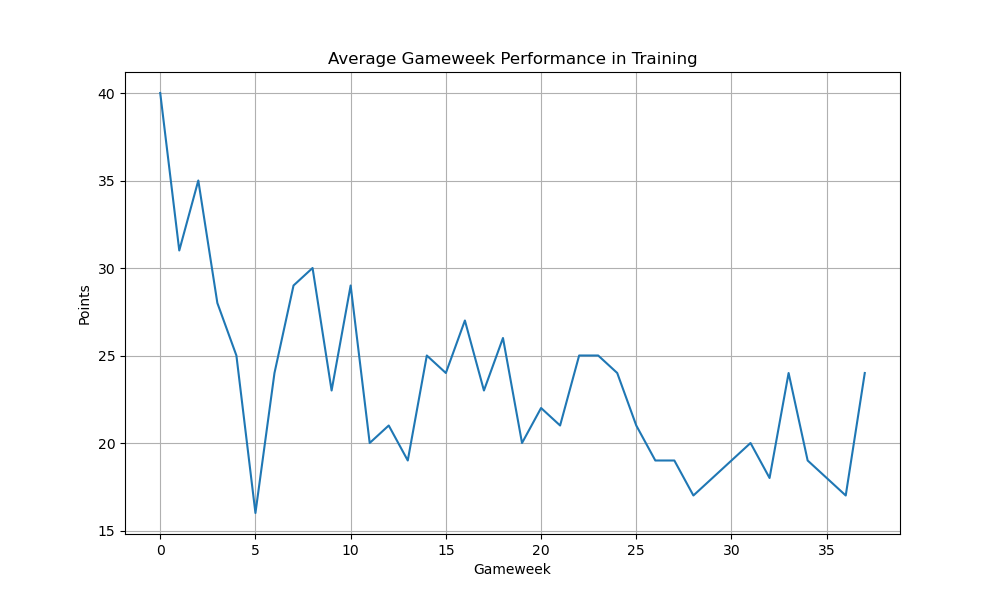
\includegraphics[width=1.0\textwidth]{figs/train_average_gameweek_performance.png}
    \vskip 0.2in
    \caption{Average points per gameweek [training]}
    \label{fig:train_average_gameweek_performance}
\end{figure}

\begin{figure}[h]
    \centering
    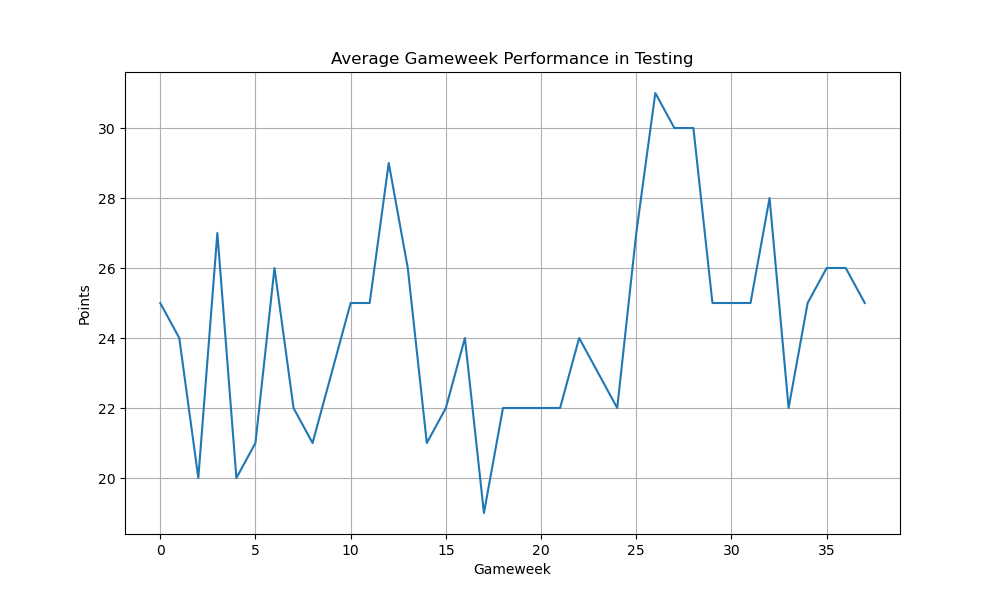
\includegraphics[width=1.0\textwidth]{figs/test_average_gameweek_performance.png}
    \vskip 0.2in
    \caption{Average points per gameweek [testing]}
    \label{fig:test_average_gameweek_performance}
\end{figure}

\section{Algorithm Analysis}
The main parameters that I experimented with while training my agent were the number of actions $a$ and the future reward discount factor $\lambda$. There was no significant change in points while varying the $a$. This likely suggests that my simplified action space with dynamically maintained subsets was effective regardless of size through periodic replacement of the weakest members as discussed in \ref{action_space}. This observation might further suggest that my agent sufficiently explored promising team selections through VPI, reinforcing the approach taken by Matthew et al. \cite{matthews2012}.

However, I found that a discount factor of 0.5 resulted in the highest average points during testing as discussed in \ref{fig:learning_curve_0.5}. A discount factor of 0.9 showed great promise during the initial episodes by quickly dwindled off, while the agent with the 0.5 discount factor closed off strongly after training with about 1130 points. The high discount factor (0.9) placed greater importance on future rewards, leading to an excessive focus on long-term potential at the expense of immediate points. A balanced discount factor (0.5) allowed the agent to give moderate importance to both immediate rewards and future potential. This allowed it to adapt better to the changing dynamics of the 2023/24 season, especially the complex blank and double gameweeks in the latter part of the season.

\begin{figure}[h]
    \centering
    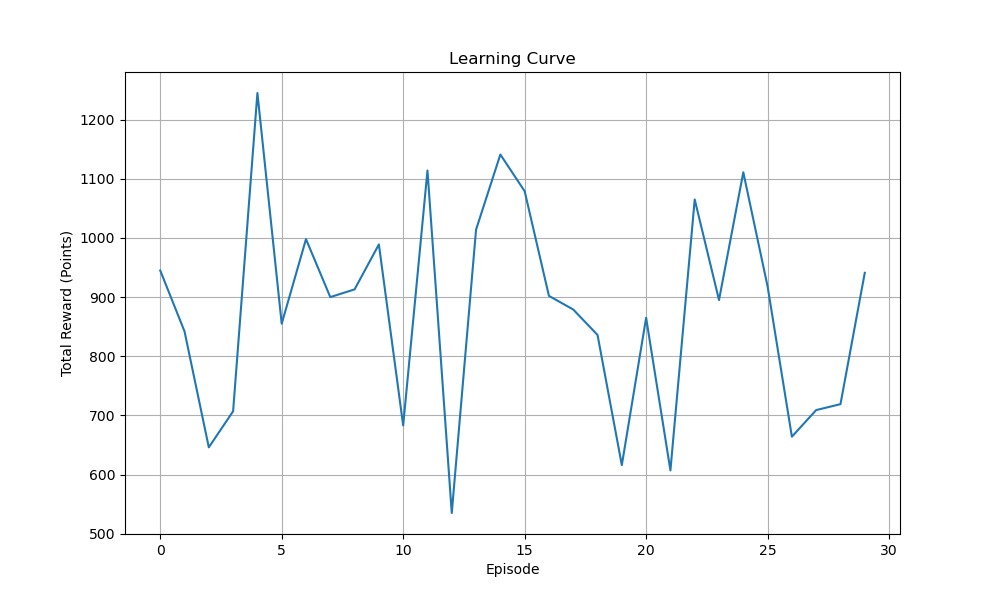
\includegraphics[width=1.0\textwidth]{figs/learning_curve_0.3.png}
    \vskip 0.2in
    \caption{Agent learning curve with a discount factor of 0.3}
    \label{fig:learning_curve_0.3}
\end{figure}

\begin{figure}[h]
    \centering
    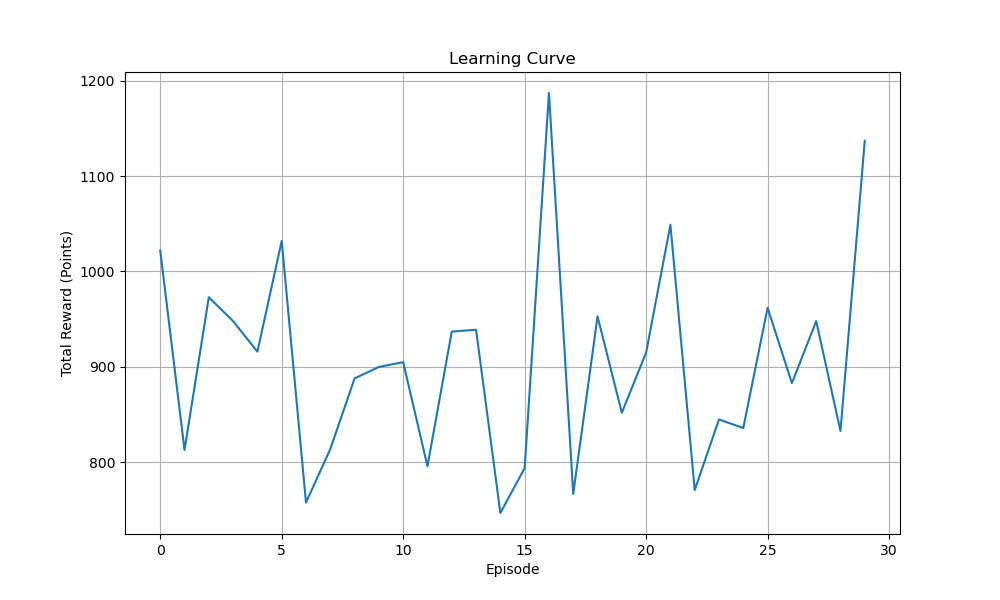
\includegraphics[width=1.0\textwidth]{figs/learning_curve_0.5.png}
    \vskip 0.2in
    \caption{Agent learning curve with a discount factor of 0.5}
    \label{fig:learning_curve_0.5}
\end{figure}

\begin{figure}[h]
    \centering
    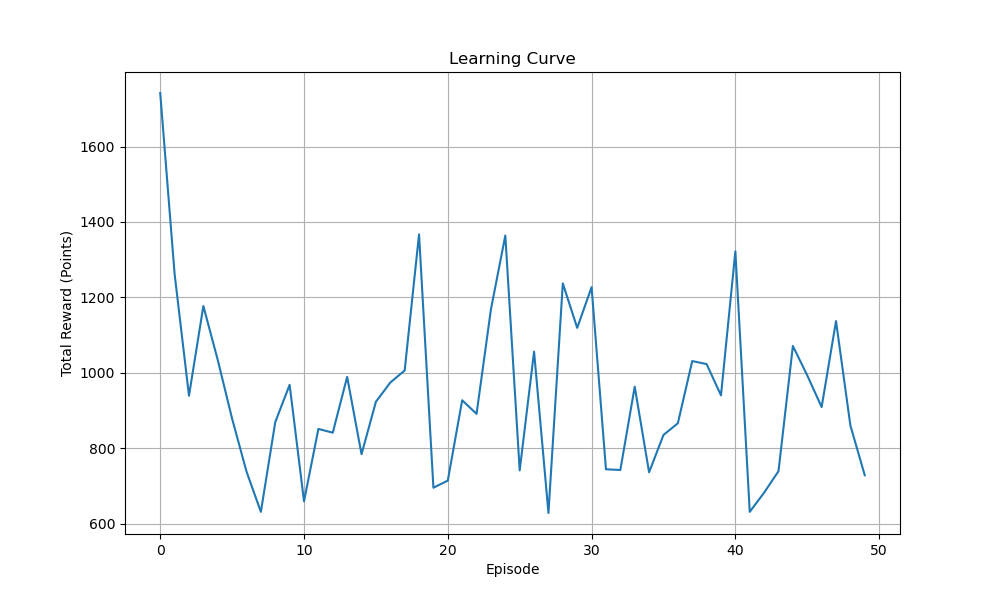
\includegraphics[width=1.0\textwidth]{figs/learning_curve_0.9.png}
    \vskip 0.2in
    \caption{Agent learning curve with a discount factor of 0.9}
    \label{fig:learning_curve_0.9}
\end{figure}


\chapter{Related Work} \label{ch:relatedwork}
Research at the intersection of artificial intelligence and fantasy sports has grown substantially over the past decade, with approaches ranging from statistical modeling to sophisticated reinforcement learning techniques.

Central to my methodology is the Bayesian modeling of player abilities. Dixon and Coles (1997) pioneered this field with their Bayesian model for football match outcomes, accounting for attacking and defensive strengths of teams while incorporating home advantage \cite{dixon1997}. Their model has become a foundation for football prediction systems and informed my fixture simulation component.

Foundational work on FPL team formation was done in the seminal paper by Matthews, Ramchurn, and Chalkiadakis (2012) establishing the first comprehensive AI framework for fantasy football management \cite{matthews2012}. Their work "Competing with Humans at Fantasy Football: Team Formation in Large Partially-Observable Domains" laid the groundwork for modeling the FPL team selection problem as a Belief-State Markov Decision Process. The authors demonstrated that an AI agent could perform at the top 0.2\% of approximately 2.5 million human competitors, despite functioning under uncertainty about player performances. Their approach utilized Bayesian Q-learning with Value of Perfect Information (VPI) exploration to balance immediate rewards with long-term planning. While groundbreaking, Matthews et al. relied heavily on the use of wildcard chips at predetermined gameweeks - 8 and 24 - to optimize team value and selection. This paper deliberately constraints the agent to operate without special chips, thereby testing its ability to navigate the FPL season through standard weekly transfers only. Furthermore, my model extends their approach by incorporating team-specific formations and training on a significantly larger dataset, spanning seven seasons (2016/17 - 2022/23) rather than just a single season.

Beyond reinforcement learning, numerous researchers have explored purely statistical approaches to fantasy sports optimization. Bonomo, Durán, and Marenco (2014) applied mathematical programming techniques to fantasy team selection, using integer linear programming to identify optimal squads within budget constraints \cite{bonomo2014}. Their model, while effective for single-gameweek optimization, lacked the capacity for sequential planning that reinforcement learning provides.

\chapter{Conclusions} \label{ch:conclusion}
I set out to explore whether a reinforcement learning agent could effectively manage a Fantasy Premier League Team while operating under constraints that reflect the challenges faced by casual managers, particularly those in different time zones from the United Kingdom. Specifically, I wanted to find out how such an agent would perform compared to the average FPL manager and whether it could achieve competitive results without replying on special chips.

Contrary to initial expectations, my constrained Bayesian Q-learning agent performed below the baseline average human managers across the season. The deliberate limitation of using only one free transfer per gameweek, while reflecting realistic constraints for casual managers, significantly hampered the agent's ability to adapt to the dynamic EPL environment. Therefore, the FPL agent struggled to recover from sub-optimal decisions made early in the season. The agent's performance particularly suffered during the irregular schedule periods, including Blank Gameweeks and Double Gameweeks. These periods require specialized strategies that proved difficult for our constrained reinforcement learning approach to discover autonomously.


\chapter{Future Work} \label{ch:futurework}
This paper has several limitations that point to promising directions for future work. 

\begin{itemize}
    \item \textbf{Alternative learning approaches}: Future work could explore deep reinforcement learning approaches that might better capture complex patterns in player and team performances, potentially improving an agent's adaptability to novel season dynamics.
    \item \textbf{Hybrid Decision Systems}: Developing systems that combine reinforcement learning with rule-based heuristics for special situations (like Blank or Double Gameweeks) could address the specific weaknesses identified in our pure reinforcement learning approach.
    \item \textbf{Social Dimension Integration}: Incorporating competitive dynamics and \\mini-league considerations could better align the agent's goals with the social \\aspects that motivate many FPL participants.
\end{itemize}

While the results did not meet my initial performance expectations, they provide valuable insights into both the potential and limitations of AI in fantasy sports management. The underperformance of my agent compared to average human managers does not invalidate my approach but rather highlights the complexity of the FPL domain and the challenges of operating under realistic constraints.


\printbibliography

\appendix
\chapter{Appendix Title} \label{ch:appendices}
Instructions on how to reproduce your experiment.
Anything that is not covered at the main but you want to add. Additional plots/results, etc.  

\end{document}

